\section{Containerisering}
\label{sec:docker}

VideoAPI distribueres som en Docker-container. Hele driftsmiljøet, inkludert API, metrikkinnsamling og dashboard, orkestreres av en enkelt \texttt{compose.yaml} i prosjektets rot. Målet med oppsettet er at en hvilken som helst Linux-VM med Docker installert skal kunne starte hele stacken med én kommando, samtidig som tjenestene kjører isolert fra hverandre og uten unødvendige privilegier. Dette oppfyller krav I1.1 \cite{hdo_kravspec} om containerisert leveranse.

\subsection{Image-bygging}
\label{subsec:docker-image}

Dockerfilen til VideoAPI er bygd som et flertrinns-image (multi-stage build) for å holde det endelige imaget lite og fritt for byggeverktøy, som vist i kodeliste~\ref{lst:dockerfile}. Første trinn, \texttt{base}, baseres på \url{mcr.microsoft.com/dotnet/aspnet:10.0} og legger til \texttt{curl} slik at containerens egen helsesjekk kan polle API-et. Andre trinn, \texttt{publish}, bruker det fullstendige .NET 10 SDK-imaget til å gjenopprette pakker og publisere applikasjonen i Release-konfigurasjon. Det ferdige \texttt{final}-trinnet kopierer kun den publiserte utdataen inn i runtime-imaget og setter \texttt{USER \$APP\_UID}, slik at prosessen kjører som en ikke-privilegert bruker. Dette er en anbefalt praksis i offisielle .NET-images for å redusere angrepsflaten \cite{aspnet_rootless}.

\begin{lstlisting}[
    language={BASH},
    label=lst:dockerfile,
    caption={Flertrinns Dockerfile for HDO-VideoAPI}
]
# HDO-VideoAPI/Dockerfile

# Trinn 1: Runtime-base med curl for helsesjekk
FROM mcr.microsoft.com/dotnet/aspnet:10.0 AS base
RUN apt-get update && apt-get install -y --no-install-recommends curl && rm -rf /var/lib/apt/lists/*
WORKDIR /app
EXPOSE 8080
EXPOSE 8443

# Trinn 2: Bygg og publiser med fullstendig SDK
FROM mcr.microsoft.com/dotnet/sdk:10.0 AS publish
ARG BUILD_CONFIGURATION=Release
WORKDIR /src
COPY ["HDO-VideoAPI.csproj", "./"]
RUN dotnet restore "HDO-VideoAPI.csproj"
COPY . .
RUN dotnet publish "HDO-VideoAPI.csproj" -c $BUILD_CONFIGURATION -o /app/publish /p:UseAppHost=false

# Trinn 3: Kopier kun publisert output inn i runtime-imaget
FROM base AS final
WORKDIR /app
COPY --from=publish /app/publish .
USER $APP_UID   # Kjør som ikke-privilegert bruker
ENTRYPOINT ["dotnet", "HDO-VideoAPI.dll"]
\end{lstlisting}

Filtreringen skjer via \texttt{.dockerignore}, som ekskluderer \texttt{.git/}, \texttt{.env}, \texttt{bin/}, \texttt{obj/}, lokale IDE-filer og hemmeligheter. Det forhindrer at sensitive verdier eller utvikleroppsett havner i imaget.

\subsection{Compose-stack}
\label{subsec:docker-compose}

Stacken som defineres i \texttt{compose.yaml} består av tre tjenester som alle deler et internt Docker-nettverk og kan referere til hverandre på tjenestenavn. Tabell~\ref{tab:compose-services} viser tjenestene og hvordan de eksponeres mot host.

\begin{table}[H]
\centering
\caption{Tjenester i Compose-stacken for HDO-VideoAPI.}
\label{tab:compose-services}
\begin{tabular}{l l l l}
\toprule
\textbf{Tjeneste} & \textbf{Image} & \textbf{Portmapping} & \textbf{Formål} \\
\midrule
\texttt{hdo-videoapi} & bygd lokalt fra \texttt{Dockerfile} & 80:8080, 443:8443 & API mot omverdenen \\
\texttt{prometheus}   & \texttt{prom/prometheus:latest}     & 9090:9090         & Skraping av metrikker \\
\texttt{grafana}      & \texttt{grafana/grafana:latest}     & 3000:3000         & Visualisering \\
\bottomrule
\end{tabular}
\end{table}

\newpage

% API-tjenesten lytter internt på 8080 (HTTP) og 8443 (HTTPS), og videresendes på host til standardportene 80 og 443. TLS-sertifikater monteres skrivebeskyttet fra hostens \texttt{./certs/}-katalog inn til \texttt{/app/certs} i containeren, slik at sertifikater kan rotere uten at bildet må bygges på nytt. Hemmeligheter (API-nøkler, Keycloak-secrets, Grafana-passord) injiseres via \texttt{env\_file: .env} og forblir utenfor bildet og versjonskontrollen.

\texttt{hdo-videoapi} lytter internt på 8080 (HTTP) og 8443 (HTTPS), og videresendes på host til standardportene 80 og 443. TLS-sertifikater monteres skrivebeskyttet fra hostens \texttt{./certs/}-katalog inn til \texttt{/app/certs} i containeren, slik at sertifikater kan rotere uten at bildet må bygges på nytt. Hemmeligheter injiseres enten direkte via \texttt{env\_file: .env} (\texttt{hdo-videoapi} jf.\ kodeliste~\ref{lst:compose-api}) eller via \texttt{environment:}-nøkler med Compose-variabelinterpolasjon fra \texttt{.env} (\texttt{grafana} jf.\ kodeliste~\ref{lst:compose-observability}), slik at ingen hemmeligheter havner i imaget eller versjonskontrollen.

%Hemmeligheter (API-nøkler, Keycloak-secrets, Grafana-passord) injiseres via \texttt{env\_file: .env} og forblir utenfor bildet og versjonskontrollen (jf.\ kodeliste~\ref{lst:compose-api}).

\begin{lstlisting}[
    language=YAML,
    label=lst:compose-api,
    caption={Compose-konfigurasjon for \texttt{hdo-videoapi}}
]
# HDO-VideoAPI/compose.yaml

services:
  hdo-videoapi:
    build: { context: ., dockerfile: Dockerfile }
    restart: unless-stopped
    ports:
      - "80:8080"
      - "443:8443"
    volumes:
      - ./certs:/app/certs:ro     # TLS-sertifikater, skrivebeskyttet
    env_file: .env                # Hemmeligheter
    healthcheck:
      test: ["CMD", "curl", "-f", "http://localhost:8080/health/live"]
      interval: 10s
      timeout: 5s
      retries: 5
      start_period: 15s
    # ... (deploy konfig)

    # ... (promethues og grafana)
\end{lstlisting}

% Prometheus konfigureres av \texttt{prometheus.yml}, som definerer ett skrape-job mot \\ \url{hdo-videoapi:8080/metrics} med 15 sekunders intervall. Siden tjenestene deler nettverk, kan Prometheus nå API-et på tjenestenavnet uten DNS-oppsett. Grafana provisjoneres automatisk fra \texttt{./grafana-provisioning/} ved oppstart, slik at dashboards og datakilder gjenopprettes også når volumet tilbakestilles.

\subsection{Tilstandshåndtering og oppstartsrekkefølge}
\label{subsec:docker-state}

% Selv om VideoAPI selv er tilstandsløs (jf.\ krav I1.2 \cite{hdo_kravspec}), skal Prometheus sine egne tidsserier og Grafanas konfigurasjon overleve omstart av containerne. Begge tjenestene bruker derfor navngitte Docker-volumer (\texttt{prometheus\_data} og \texttt{grafana\_data}) som ligger utenfor containerens skrivelag. Prometheus konfigureres av \texttt{prometheus.yml} med ett skrape-job mot \texttt{hdo-videoapi:8080/metrics} med 15 sekunders intervall (jf. delkapittel~\ref{subsec:obs-prom}), og Grafana provisjoneres automatisk fra \texttt{./grafana-provisioning/} ved oppstart (jf. delkapittel~\ref{subsec:obs-graf}).

% Selv om VideoAPI selv er tilstandsløs (jf.\ krav I1.2 \cite{hdo_kravspec}), skal Prometheus sine egne tidsserier og Grafanas konfigurasjon overleve omstart av containerne. Begge tjenestene bruker derfor navngitte Docker-volumer (\texttt{prometheus\_data} og \texttt{grafana\_data}) som ligger utenfor containerens skrivelag. Figur~\ref{fig:compose_startup} illustrerer oppstartsrekkefølgen.

Selv om VideoAPI selv er tilstandsløs (jf.\ krav I1.2 \cite{hdo_kravspec}), skal Prometheus sine egne tidsserier og Grafanas konfigurasjon overleve omstart av containerne. Begge tjenestene bruker derfor navngitte Docker-volumer (\texttt{prometheus\_data} og \texttt{grafana\_data}) som ligger utenfor containerens skrivelag.

Tjenestene starter i kontrollert rekkefølge slik at metrikkstacken ikke logger feil før API-et er klart, som illustrert i figur~\ref{fig:compose_startup}.

\begin{figure}[H]
    \centering
    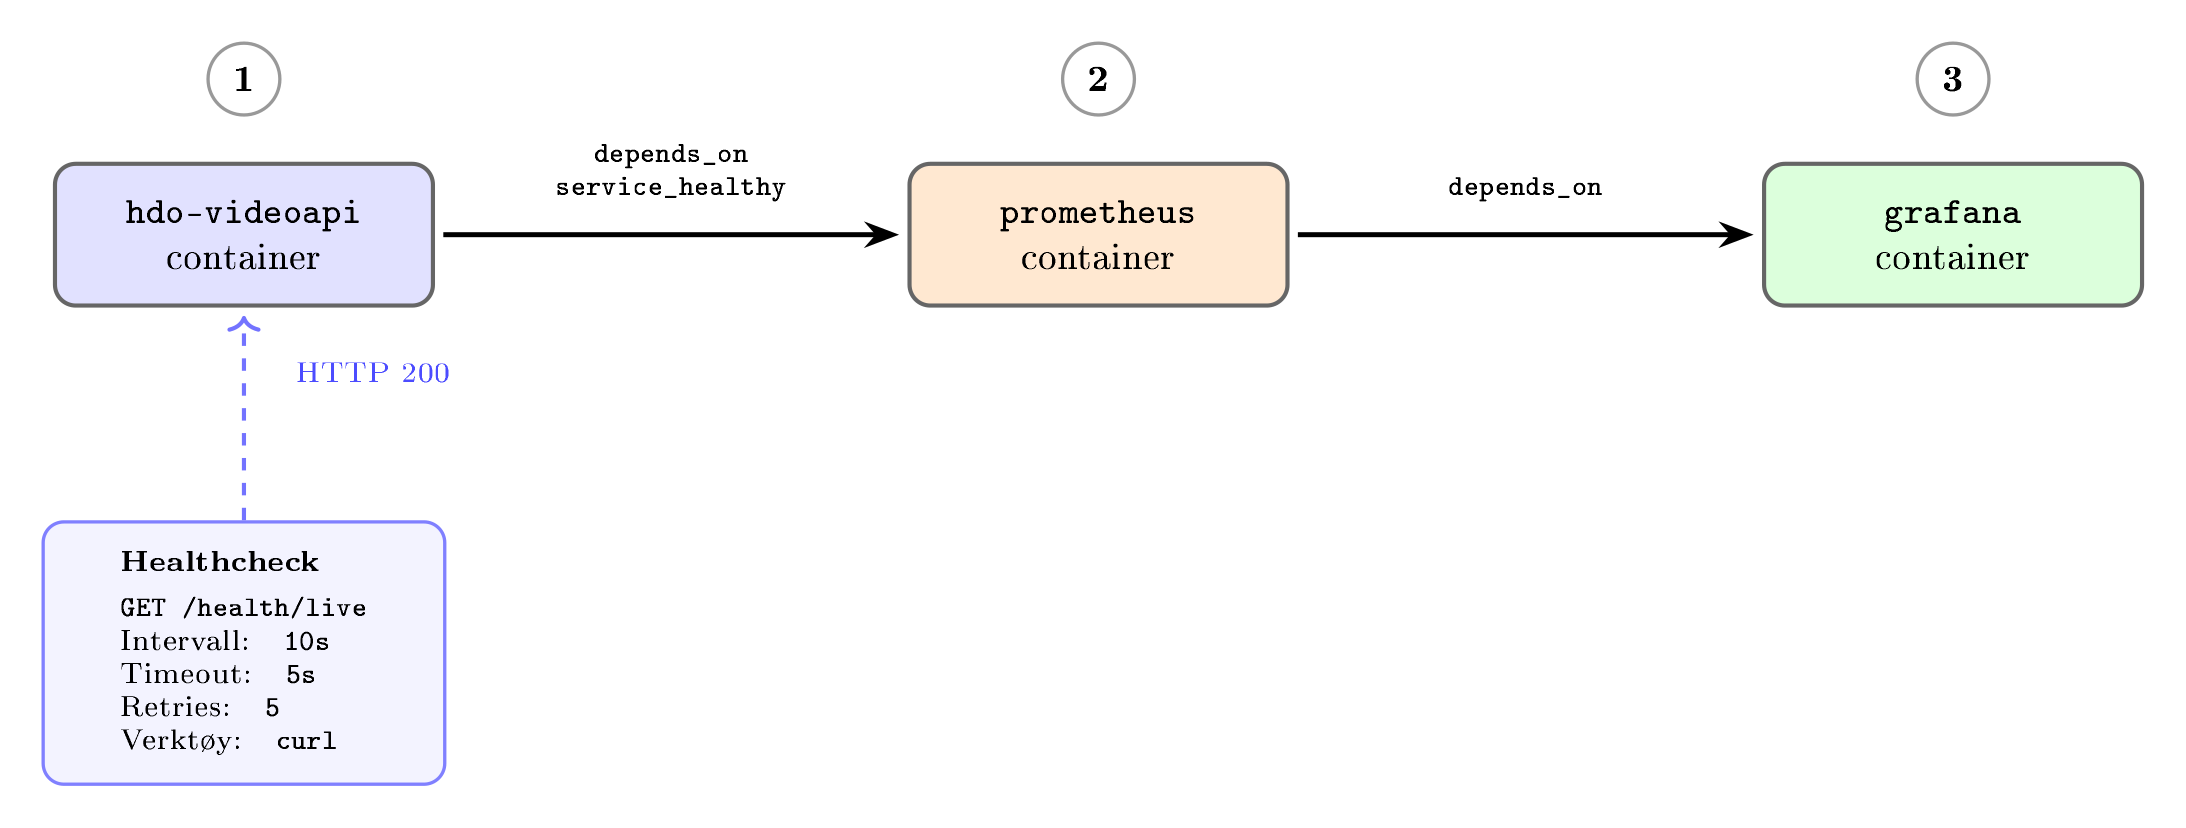
\includegraphics[width=1\linewidth]{figures/compose_startup.png}
    \caption{Kontrollert oppstartsrekkefølge i Docker Compose-stacken. 
             \texttt{prometheus} og \texttt{grafana} starter ikke før 
             \texttt{hdo-videoapi} rapporterer \texttt{healthy} på 
             \texttt{/health/live}}
    \label{fig:compose_startup}
\end{figure}

\newpage

% Tjenestene starter i kontrollert rekkefølge slik at metrikkstacken ikke logger feil før API-et er klart. \texttt{prometheus} har \texttt{depends\_on: hdo-videoapi} med betingelsen \texttt{service\_healthy}, og \texttt{grafana} har \texttt{depends\_on: prometheus}. Det betyr at Prometheus først starter når API-ets \texttt{/health/live}-endepunkt returnerer HTTP-status \texttt{200 OK}, og at Grafana først starter etter Prometheus. Selve helsesjekken er definert i Compose-filen og bruker \texttt{curl} til å treffe \texttt{/health/live} hvert tiende sekund med fem sekunders timeout og opp til fem nye forsøk før containeren markeres som \texttt{unhealthy}.

% Tjenestene starter i kontrollert rekkefølge slik at metrikkstacken ikke logger feil før API-et er klart (jf.\ kodeliste~\ref{lst:compose-observability}). \texttt{prometheus} har \texttt{depends\_on: hdo-videoapi} med betingelsen \texttt{service\_healthy}, og \texttt{grafana} har \texttt{depends\_on: prometheus}. Det betyr at Prometheus først starter når API-ets \texttt{/health/live}-endepunkt returnerer HTTP-status \texttt{200 OK}, og at Grafana først starter etter Prometheus. Selve helsesjekken bruker \texttt{curl} til å treffe \texttt{/health/live} hvert tiende sekund med fem sekunders timeout og opp til fem nye forsøk før containeren markeres som \texttt{unhealthy}.

\texttt{prometheus} har \texttt{depends\_on: hdo-videoapi} med betingelsen \texttt{service\_healthy}, og \texttt{grafana} har \texttt{depends\_on: prometheus}. Det betyr at Prometheus først starter når API-ets \texttt{/health/live}-endepunkt returnerer HTTP-status \texttt{200 OK}, og at Grafana først starter etter Prometheus. Grafana venter kun på at Prometheus er startet (\texttt{service\_started}) fordi Grafana ikke er avhengig av at Prometheus allerede skraper data -- det holder at prosessen er oppe og klar til å ta imot spørringer. Selve helsesjekken bruker \texttt{curl} til å treffe \texttt{/health/live} hvert tiende sekund med fem sekunders timeout og opp til fem nye forsøk før containeren markeres som \texttt{unhealthy} (jf. kodeliste~\ref{lst:compose-api}). Kodeliste~\ref{lst:compose-observability} viser Compose-definisjonene for \texttt{prometheus} og \texttt{grafana}, med volumer og \texttt{depends\_on}-betingelser.

\begin{lstlisting}[
    language=YAML,
    label=lst:compose-observability,
    caption={Compose-konfigurasjon for Prometheus og Grafana}
]
# HDO-VideoAPI/compose.yaml

services:
  # ... (hdo-videoapi)
    
  prometheus:
    image: prom/prometheus:latest
    restart: unless-stopped
    ports:
      - "9090:9090"
    volumes:
      - ./prometheus.yml:/etc/prometheus/prometheus.yml # Scrape-konfigurasjon
      - prometheus_data:/prometheus                     # Persistent lagring
    depends_on:
      hdo-videoapi:
        condition: service_healthy  # Starter etter at API-et er healthy
    # ... (deploy konfig)

  grafana:
    image: grafana/grafana:latest
    restart: unless-stopped
    ports:
      - "3000:3000"
    volumes:
      - grafana_data:/var/lib/grafana                       # Persistent lagring
      - ./grafana-provisioning:/etc/grafana/provisioning    # Auto-provisjonering
    environment:
      - GF_SECURITY_ADMIN_USER=${GRAFANA_USER}
      - GF_SECURITY_ADMIN_PASSWORD=${GRAFANA_PASSWORD}
      - GF_PLUGINS_AUTO_UPDATE_ENABLED=false
    depends_on:
      prometheus:
        condition: service_started
    # ... (deploy konfig)

# Navngitte volumer for persistens
volumes:
  prometheus_data:
  grafana_data:
\end{lstlisting}

Alle tre tjenestene bruker \texttt{restart: unless-stopped}, slik at de kommer opp igjen automatisk etter krasj eller VM-omstart, men forblir nede dersom de er manuelt stoppet av driftspersonell.

\subsection{Ressurskontroll og sikkerhet}
\label{subsec:docker-security}

For å hindre at en enkelt container uttømmer hostens ressurser, settes \texttt{deploy.resources.limits} per tjeneste: VideoAPI begrenses til 512~MB minne og én CPU-kjerne, Prometheus til 256~MB, og Grafana til 1~GB. Verdiene er forankret i den observerte ressursbruken under last- og integrasjonstesting (se delkapittel~\ref{sec:eval-infrastruktur}), og gir tydelige grenser for systemovervåkningen.

Sikkerhetsmessig hviler stacken på flere lag. API-et selv kjører som ikke-privilegert bruker (\texttt{UID 1654} i .NET-imaget), TLS-sertifikatene monteres skrivebeskyttet, hemmeligheter ligger kun i \texttt{.env}, og \texttt{appsettings.Docker.json} overstyrer Kestrel-endepunktene til å lytte på portene containeren eksponerer og peker sertifikatstiene til volummonteringen fra host -- filen inneholder ingen hemmeligheter. Prometheus eksponerer ingen autentisering ut av boksen og er derfor tilgjengelig uten tilgangskontroll; Grafana beskyttes av eget brukernavn og passord satt via miljøvariabler.

\subsection{Driftsflyt}
\label{subsec:docker-ops}

Med stacken på plass blir hele drifts-livssyklusen redusert til et fåtall kommandoer. Hele stacken bygges og startes i bakgrunnen med \texttt{docker compose up -d -{}-build}, og en enkelttjeneste kan rebygges med samme kommando etterfulgt av tjenestenavnet. \texttt{docker compose down} stopper alle containerne, mens \texttt{docker compose down -v} i tillegg sletter de navngitte volumene. Logger fra en spesifikk tjeneste følges med \texttt{docker compose logs -f <tjeneste>}. Samspillet mellom helsesjekk, oppstartsrekkefølge og volumer muliggjør at en VM kan rebootes uten manuelt inngrep. Tjenestene startes i riktig rekkefølge og gjenoppretter tidligere tilstand.